	%------------------第一章---------------------------
	\newpage
	\section{绪论}
    \subsection{超声波接近传感器的研究背景和意义}
    \subsubsection{超声波接近传感器的发展}
    超声波接近传感器是一种常用的非接触式测距传感器,它能够将物体到传感器的距离转化为电信号,实现物体的远近判断。超声波接近传感器广泛应用于工业自动化、机器人、无人驾驶等领域。随着技术的发展,超声波接近传感器的性能不断得到提高。    
    超声波接近传感器的发展经历了三个阶段。第一代超声波接近传感器采用固定式超声波传感器,能够实现对物体距离的测量,但是存在精度不高、抗干扰能力弱等问题。第二代超声波接近传感器采用微机处理技术和数字滤波技术,在一定程度上提高了抗干扰能力。第三代采用了新型材料和新技术,如MEMS技术、FPGA技术等,进一步提高了系统的测量精度、稳定性。
    \subsubsection{超声波接近传感器国内外研究现状}
    \paragraph{国内研究现状}
	国内科研人员在超声波接近传感器上取得了突破性进展,主要集中在回波检测、超声换能器设计、发射脉冲选取等方面。
	
	在超声波换能器设计方面,2004年,通过对Vmos场效应管开关元件发射电路进行分析,矿业研究所的马庆云等研究发现,触发脉冲对超声波换能器的发射功率产生影响,最大发射功率对应的触发脉冲宽度是其谐振周期的$\frac{1}{2}$\upcite{超声波测距传感器的研究6}。这一发现对新型超声波换能器发射电路的研究具有指导作用,因为它可以克服传统调频超声波系统必须使用宽带超声传感器的问题,通过调整触发脉冲宽度来控制发射功率,从而实现对超声波发射信号的精确控制。
	
	2005年,李希胜等人在北京科技大学进行了一项研究,即窄带调频超声波距离检测。该技术不仅能够以极低的瞬时超声波功率实现极高的平均发射功率,而且还可以通过普通的超声波传感器实现,大大降低了传感器的成本。
	
	2006年,潘仲明对大检测范围超声波接近传感器进行了研究。该研究在谐振频率为23.5$kHz$基础上,研发出一种新型超声波接近传感器,其作用距离可以达到$31m$以上,测量误差低于$3\%$\upcite{超声波测距传感器的研究7}。
		
	在发射脉冲选取方面,程晓畅在2006年提出了一种基于雷达信号处理中的脉冲压缩技术的超声波发射脉冲选取方法,使用伪随机二进制序列来提供超声波发射的压缩信号,获得更高的信号功率和更小的脉冲宽度,从而提高了超声波信号的分辨率和检测精度\upcite{超声波测距传感器的研究8}。这种方法有效地解决了传统超声波检测中信号功率不足、信号宽度大等问题,为超声波检测技术的提高提供了重要的理论基础和实验支持。
	
	2008年,在嵌入式领域,杜晓同时考虑到测距量程和精度,利用$40kHz$与$20kHz$两种频率的超声波进行测距,将脉冲压缩技术很好的与双频超声测距技术相融合,使超声波接近传感器即可以增加检测范围,又能提高检测分辨率\upcite{超声波测距传感器的研究9}。
		
	2007年,陈平等人通过改良测距算法,设计了一种液位检测传感器。该超声波传感器考虑了温度对声速的影响,通过检测温度来对声速进行调整补偿,从而提高了检测分辨率。
	
	在机器人视觉领域,田志宏在2007年设计了一种可智能避障的自动轮椅车,并在传感器技术学报上发表了相关成果\upcite{超声波测距传感器的研究10}。王洪青研究出了一种并行超声波测距系统,该系统在各个方向安装传感器,实现了多传感器数据融合、实时检测距离的效果。
	
    \paragraph{国外研究现状}
	同样,超声波接近传感器在国外也有了很大的发展。
	
	2013年2月,在伦敦帝国大学,Joseph Jackson,Rahul Summa等采用渡越时间法来进行超声波测距,该方法被应用于机器人、物体结构探测领域的研究\upcite{超声波测距传感器的研究11}。
	
	2010年12月,里斯本大学的研究人员Ricard Queiros和Francisc Corre Alegria提出了一种新型的超声波接近传感器测距方法。该方法利用了交叉相关联和正弦发生器技术,提高了传感器的精度。交叉相关技术通过将发送信号与接收信号相融合,检测超声波在空气中传播的时间,从而精确测量距离;正弦发生器则可以检测超声波传播过程中的相移,进而提高测距的分辨率。
	
	2011年,JiDe Huang和Chih Kung Lee在康奈尔大学提出了一种新的高精度超声波测距系统,该系统采用基于峰值检测和干涉技术的方法。该超声波测距系统的特点是通过硬件设计提高了测距系统的精度,而不依赖于复杂的算法,不仅提高了传感器的精度,还没有使得成本增加。\upcite{超声波测距传感器的研究14}。
	
    
    \subsubsection{超声波接近传感器的研究意义}
    TUSS4470芯片作为一种新型的超声波传感器芯片,具有高精度、低功耗和多种工作模式等特点,可以满足现代工业和自动化控制对于测量、检测、控制和导航等方面的需求。因此,基于TUSS4470芯片的超声波接近传感器的研究成为了一个热门话题,其可以应用于智能家居、无人机、自动驾驶车辆、机器人等领域,具有广阔的应用前景和市场前景。\par
    此外,在传统的超声波驱动控制电路中,一般是采用模拟电路或者单片机来控制。由模拟电路驱动的超声波传感器抗干扰性差,而由单片机驱动的超声波传感器,由于其使用外部中断触发的机制,导致无法精确控制时序逻辑,从而难以达到与超声探头匹配的驱动频率,而超声波传感器的检测精度直接取决于其发出脉冲宽度的精度\upcite{CPLD在超声波传感器驱动控制电路中},当脉冲宽度无法匹配时将使得传感器的精度降低,因此使用CPLD芯片控制产生精确的脉冲宽度对提高传感器的检测精度有着十分重要的意义。\par
    本设计采用型号为EPM240T100C5N的MAX II系列芯片,它是一种高集成度、电可擦除、CMOS宏阵列可编程逻辑器件\upcite{基于STM32和超声波测距的倒车雷达预警系统设计},可以产生ns级别的控制信号\upcite{CPLD芯片介绍},配合TUSS4470超声驱动芯片,可精确控制发送脉冲的次数、频率以及脉冲宽度。同时,CPLD芯片编程采用时序逻辑,发送、接收、检测脉冲信号的时间可进行精确控制,这让超声检测策略可以变得更加丰富合理。
    \subsection{超声波接近传感器的原理}
    \subsubsection{超声波介绍}
      超声波是一种弹性机械波,可以在气体、液体和固体中传播。人们可以听到的声音频率范围是$20Hz\sim20kHz$,超出该范围的声音被称为低频声波或超声波。超声波的纵向分辨率较高,对许多干扰因素如光线、电磁波都不敏感,不易受环境的影响,且超声波在遇到物体反射时,入射角和反射角近似相等,方便用于测量较近目标的距离\upcite{车载可视倒车雷达预警系统的研制}。
      
      超声波的传播方向与振动方向一致,是纵向振动的弹性机械波,其波动方程描述方法与电磁波相似,如式\ref{波动方程}所示。
    \begin{equation}
    	A=A(x)cos(\omega t+kx)
    	\label{波动方程}
    \end{equation}
	式中\quad$x$---传播距离;\par
	\quad$\omega$---频率
	\begin{equation}
		A(x)=A_0 e^{-\alpha x}
		\label{振幅方程}
	\end{equation}
	式中\quad$A(x)$---振幅;\par
		\quad$\alpha$---衰减指数
	\begin{equation}
		\alpha=a f^2
		\label{衰减指数}
	\end{equation}
	式中\quad $a$---介质常数;\par
	   \quad $f$---振动频率\par
    根据式\ref{衰减指数}我们可以得出,当频率越高时,衰减系数$\alpha$越大,传播距离越短。这是因为声波在空气里传播时,会与空气分子间存在运动摩擦,能量会被损耗。但超声波频率越高时,其指向性越强,有利于回波的反射和检测。综合考虑指向性和损耗两个指标,为达到良好的检测效果,在设计超声波接近传感器时,我们选用中心频率为$300kHz$的超声波换能器。
    \subsubsection{超声换能器的结构}
    超声换能器是一种将其它形式的能转换为超声能或是将超声能转换为其他形式的能的装置。在实际应用中,常用的超声换能器主要包括电声型和流体动力型两类\upcite{面向机器人安全避障的MEMS压电超声接近觉传感器的研究39}。
    电声型超声换能器主要包括压电换能器、磁质伸缩换能器和静电换能器三种。其中,压电换能器是最常用的一种,它利用压电效应将电能转化为机械能或将机械能转化为电能\upcite{车载可视倒车雷达预警系统的研制}。磁质伸缩换能器则是利用磁性材料的磁致伸缩效应实现能量转换,静电换能器则是利用静电场的作用实现能量转换。
    流体动力型超声换能器主要包括气体和液体两种类型。其中,气体型是利用气体流动产生的声波进行能量转换,液体型则是利用液体流动产生的声波进行能量转换。这两种传感器在实际应用中具有一定的局限性,主要是在响应频率、灵敏度、稳定性等方面存在一定的问题\upcite{车载可视倒车雷达预警系统的研制13}。\par
    压电式超声波换能器是一种电声型传感装置,它利用压电材料的特性将电能转换为机械振动,将机械振动转换为电能,是超声检测中最常用的一种传感装置,是超声波检测装置的重要组成部分。压电式超声波换能器的核心是压电晶片,它可以产生逆压电效应和正压电效应。当压电晶片接收到发射电脉冲时,逆压电效应会使晶片振动并发射超声波;而当晶片接收到超声波时,正压电效应会使晶片发生机械变形,并将其转换成相应的电信号。通常采用双压电陶瓷晶片制成超声波换能器,其中一个晶片用于发射超声波,另一个用于接收超声波\upcite{车载可视倒车雷达预警系统的研制15}。
    \begin{figure}[!h]

    	\begin{minipage}{0.5\textwidth}
    		\centering
    		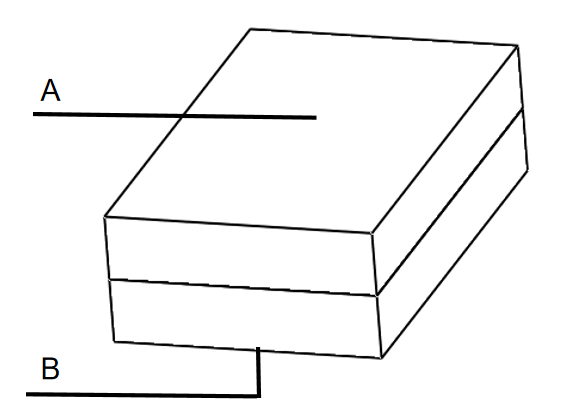
\includegraphics[height=4cm]{figure/双压电晶片示意图.png}
    		\caption{双压电晶片示意图}
    		\label{双压电晶片示意图}
    	\end{minipage}
    \begin{minipage}{0.5\textwidth}
    	\centering
    	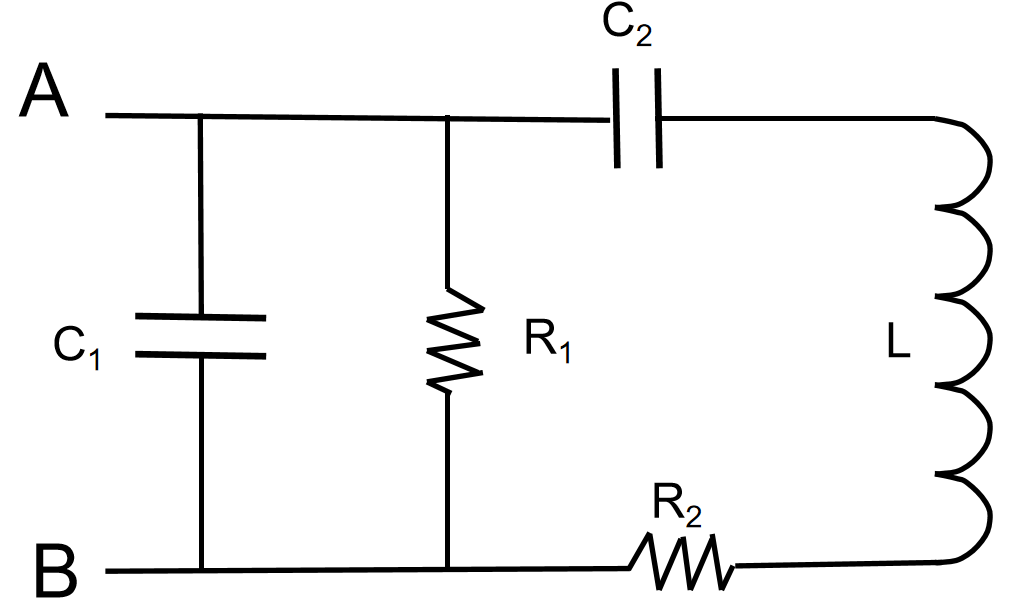
\includegraphics[height=4.25cm]{figure/双压电晶片等效电路.png}
    	\caption{双压电晶片等效电路图}
    	\label{双压电晶片等效电路图}.
    \end{minipage}
    \end{figure}

    双压电晶片如图\ref{双压电晶片示意图}所示,当在两晶片间施加交流电压时,如果电场方向与极化方向相同,则起到了增强极化作用的效果,如果电场方向与极化方向相反,则对极化作用起到了削弱的效果,利用该原理,可使压电晶片产生与交变电场频率相同的交变形变,当这种形变传递到介质中时,就产生超声波。双压电晶片的等效电路如图\ref{双压电晶片等效电路图}所示。$C_1$为静电电容,$R_1$为陶瓷材料介电损耗并联电阻,$C_2$和$L$为陶瓷材料介电损耗并联电阻,$R_2$为损耗串联电阻\upcite{51单片机超声波测距仪防撞报警倒车雷达设计}。\par

    压电陶瓷晶片有一个固定的谐振频率,即中心频率$f$。脉冲信号频率与施加交变电场频率越相近,传感器的精度就越高。当所用材料不变时,改变晶片尺寸,就可改变其中心频率,从而可以得到具有各种中心频率的超声传感器\upcite{车载可视倒车雷达预警系统的研制16}。
    超声换能器的结构如图\ref{超声换能器结构图}所示,其主要由金属网、外壳、圆锥形振子、双晶振子、底座和引脚等部分组成 。
    \begin{figure}[!h]
    	\centering
    	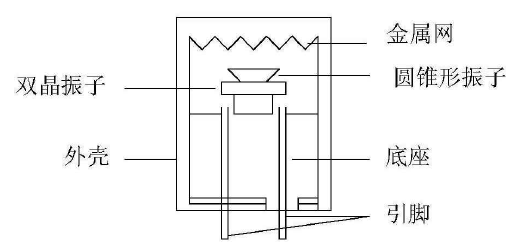
\includegraphics[width=7cm]{figure/超声换能器结构图.png}
    	\caption{超声换能器结构图}
    	\label{超声换能器结构图}
    \end{figure}
\newpage
    \subsubsection{超声波接近传感器的检测原理}
    \paragraph{连续波相位检测法(CW法))}
    连续波相位检测法的测距原理如图\ref{连续波相位检测法}所示。发射换能器和接收换能器同时发射和接收超声波信号,通过检测信号之间的相位差来获取时间延迟,并计算出传感器与障碍物之间的距离\upcite{面向机器人安全避障的MEMS压电超声接近觉传感器的研究34}。\par
    \begin{figure}[!h]
    	\centering
    	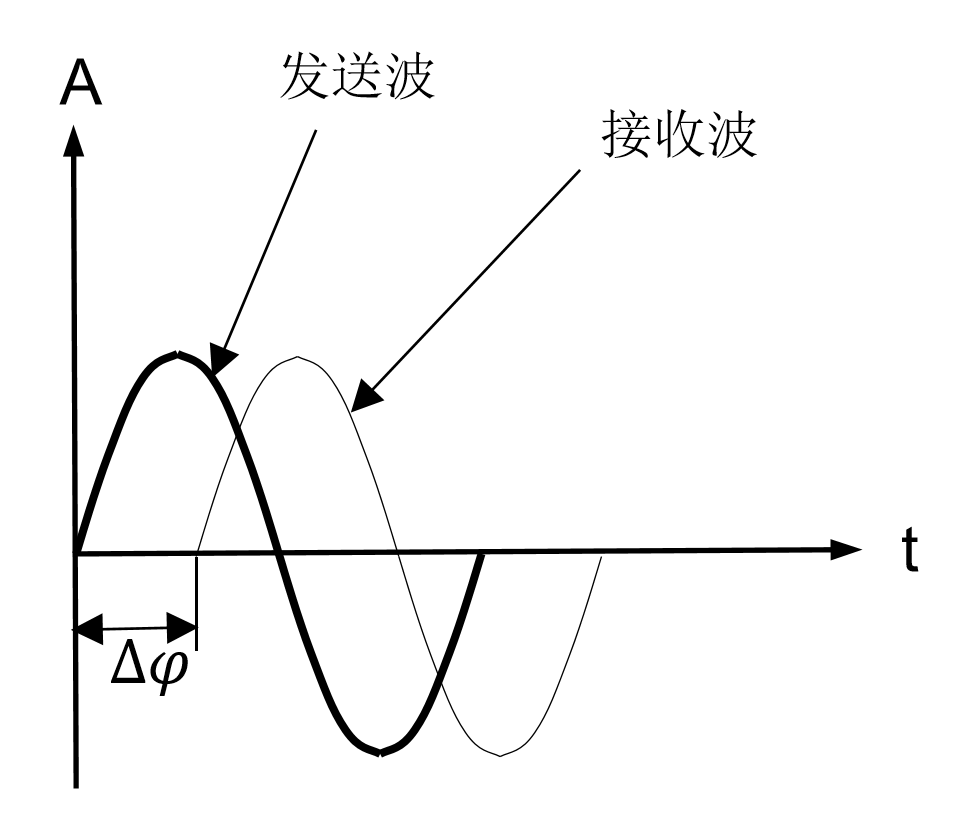
\includegraphics[width=6cm]{figure/连续波相位检测法.png}
    	\caption{连续波相位检测法}
    	\label{连续波相位检测法}
    \end{figure}\par


    假设 发射 的 声 波信 号 为 :
    \begin{equation}
    	u_1=A(x)sin(\omega t + \varphi)
    \end{equation}
式中\quad$\varphi$---初始相位角
接收到的回波信号为:
\begin{equation}
	u_2=A(x)sin(\omega t + \varphi + \omega \cdot{\frac{2D}{c}})
\end{equation}
式中\quad$c$---声速\par
发射声波与回波间的相位差为$\Delta \varphi=\frac{2D}{c}$,传感器与检测物体间的距离D为:
\begin{equation}
	D=\frac{c}{2\omega}\cdot \Delta \varphi=\frac{c}{4\pi f}\cdot(2\pi n + \varphi_i)
\end{equation}
式中\quad$n$---整周期的个数;
\quad$\varphi_i$---不完整周期的相位值。\par
虽然相位检测法的精度比较高,但处理电路的成本也高,需要设计比较复杂的处理电路才能准确地确定回波信号的相位,计算量大\upcite{面向机器人安全避障的MEMS压电超声接近觉传感器的研究35}。\par



    
    \paragraph{飞行时间法}
    飞行时间检测法又称脉冲一回波检测法(如图\ref{飞行时间检测法})。超声换能器发射一组脉冲,在遇到障碍物后脉冲进行反射,换能器在接收到反射回波时,会与发射时刻之间产生时间延迟,该时间延迟称为超声波的飞行时间$t$,飞行时间$t$与声波速度$c$和传播距离$L$有关,即$t=\frac{L}{c}$。
    \begin{figure}[!h]
    	\centering
    	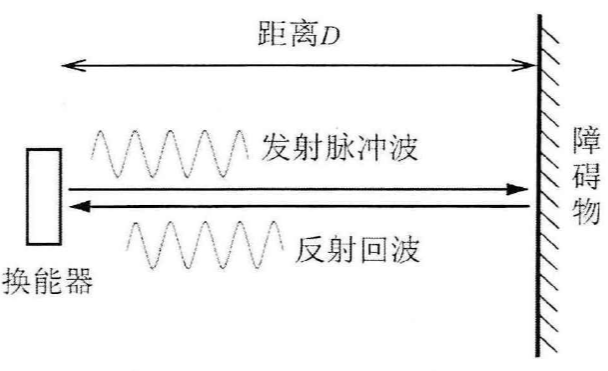
\includegraphics[width=6cm]{figure/飞行时间检测法.png}
    	\caption{飞行时间检测法}
    	\label{飞行时间检测法}
    \end{figure}\par
    飞行时间法最少使用一个换能器便可以实现超声波脉冲的发射和接受,对于自发自收的测距传感器,距离$D$的计算公式为:
    \begin{equation}
    	D=\frac{L}{2}=\frac{ct}{2}
    \end{equation}\par

	采用飞行时间检测法进行障碍物测距,如何简单准确地获得超声波自发射至接收时的飞行时间,是此方法的关键所在。获取飞行时间的方法有很多种,常见的飞行时间法有:互相关函数法、固定阈值法和包络峰值法。\par
	超声波的回波信号相较于发射信号而言,波形基本不变,但在时间上会有一定延迟,因此这两个信号具有相关性。为了准确获取超声波自发射至接收的飞行时间,可以采用相关函数法进行测量。互相关函数法是对超声波的发射信号和回波信号进行互相关函数计算,函数最大值处所对应的时刻就是收发信号相关性最大的时刻,也是回波信号的接收时刻\upcite{面向机器人安全避障的MEMS压电超声接近觉传感器的研究36}。通过计算超声波发射时刻与互相关函数最大值时刻之间的时间差,就可以准确获得超声波的飞行时间。除此之外,固定阈值法和包络峰值法也是常用的飞行时间法。\upcite{面向机器人安全避障的MEMS压电超声接近觉传感器的研究}\par
	固定阈值法是指预先设置一个确定的阈值,当接收的回波信号幅值大于此阈值时,认为此信号幅值所在时刻为回波信号的到达时刻,从而获取超声波的飞行时间。但是在回波信号达到预设阈值时,此时所确定的时刻并不是回波信号的起振时刻,具有一定的时间偏差进行时间补偿将其消除后便可获得飞行时间的估计值。阈值预设大小是固定阈值法用于测量距离的关键因素之一。在固定阈值法中,通过将预设阈值与回波信号的幅值进行比较来判断障碍物距离,而阈值的设置会直接影响到测量结果的精确度。如果阈值设置过高,当障碍物距离较远时,回波信号幅值无法达到阈值大小,导致无法获取飞行时间,从而无法准确测量距离。相反,如果阈值设置过低,噪声信号容易达到阈值大小,造成误触发,导致测量结果不可靠。此外,固定阈值法方法还存在其他问题,例如不同反射距离的回波信号波形幅值大小不同,所造成的时间偏差也不同,简单时间补偿无法获得真实飞行时间,进一步降低了测量结果的精确度。因此,虽然固定阈值法方法简单、易实现、计算量不大,但其精度不高,抗干扰能力差的缺点不能忽视。\par
	包络峰值法是一种常见的获取超声波飞行时间的方法。该方法利用回波信号包络线的峰值所在时刻来获取飞行时间。相比于固定阈值法,该方法更加准确,因为回波信号的幅值会随着传播距离的增加而发生变化,而峰值所在的位置相对回波信号的起振时刻并没有发生变化。此外,回波信号的上升时间与超声波发射信号的频率和周期有关,而与传播距离无关,这种特性也使得包络峰值法可以较好地弥补时间偏差,提高测量精度。值得一提的是,包络峰值法同样存在一些缺点,例如受噪声和杂波的影响较大,需要在实际应用中进行适当的干扰抑制和信号处理。\upcite{面向机器人安全避障的MEMS压电超声接近觉传感器的研究38}。
	       
\subsection{本设计的主要研究内容和论文结构安排}
\subsubsection{主要研究内容}
本设计针对生产线上检测钢化玻璃到位问题,设计了一种稳定性好、灵活性高、应用场景广的超声波接近传感器。
本设计的主要研究内容包括了超声波接近传感器的硬件设计、软件设计和实验设计。\par
硬件设计包括了原理图设计和PCB设计,软件设计包括了驱动芯片配置、脉冲信号产生、物体检测三个部分的程序设计以及波形仿真,实验设计部分包括了设计实验进行性能参数测试、稳定性测试和回波特性测试。

\subsubsection{论文结构安排}
本文各章节的主要内容如下:

第二章:提出了超声波接近传感器的总体设计,初步介绍各个部分的设计流程与方法步骤。然后讲解了在本设计所涉及到的检测原理。

第三章:对传感器的硬件电路设计进行研究,介绍了原理图设计和PCB设计的设计过程。原理图部分的设计分为三部分,分别为:超声波接近传感器控制电路设计、TUSS4470芯片外围电路设计、检测计数电路设计。PCB设计部分主要介绍了TUSS4470外围电路PCB设计,讲解了在PCB设计过程中遵循的几大原则,用于减小各类信号相互之间的干扰,包括了电容、二极管等器件摆放位置优先级,分离接地,铺铜规则等。

第四章:对传感器的软件设计进行研究,首先讲解了传感器所采取的检测策略,然后进行程序的总体设计,根据功能将程序分为了四个模块,分别为:控制模块、SPI模块、脉冲产生模块和检测计数模块。之后分别详细讲解了各个模块的功能、实现原理以及程序流程图。在完成了程序设计方面的工作后,又介绍了如何搭建仿真环境进行程序仿真模拟,最后,给出了仿真模拟后的波形图,并进行了分析。

第五章:设计实验测试传感器的性能以及检测策略的可行性。首先讲解了实物的焊接与调试流程,给出了调试过程中所测得的各引脚波形,然后介绍了实验所用的实验器材,包括虚拟示波器、直尺、各种板材等。最后进行实验,测试了传感器的性能参数、稳定性以及回波特性,给出了实验的结果以及后续分析。

第六章:对本设计存在的不足进行总结,提出了改进的方向,并且进行了对未来的展望。


    \subsection{本章小结}
    本章绪论主要介绍了超声波接近传感器的研究背景和意义,在研究背景中介绍了超声波接近传感器总体的发展情况以及国内外研究现状,然后引出本设计的研究意义是为了设计精度高、稳定性好的传感器。在第二节主要介绍了传感器主要涉及到的原理,包括超声波振幅衰减原理、超声换能器发射脉冲与检测回波信号的原理以及在本设计中的检测原理。在本章的最后一节,则是介绍了本设计的主要研究内容和论文结构安排
    ,并且简单介绍了后几章所包含的内容。